\documentclass[12pt,tikz]{standalone}

\usepackage{graphicx}
\usetikzlibrary{positioning}
\begin{document}
\fontsize{16}{20}\selectfont

\newcommand{\state}[2]{%
  $s = $ \texttt{#1}\\
  $p = $ \texttt{#2}
}

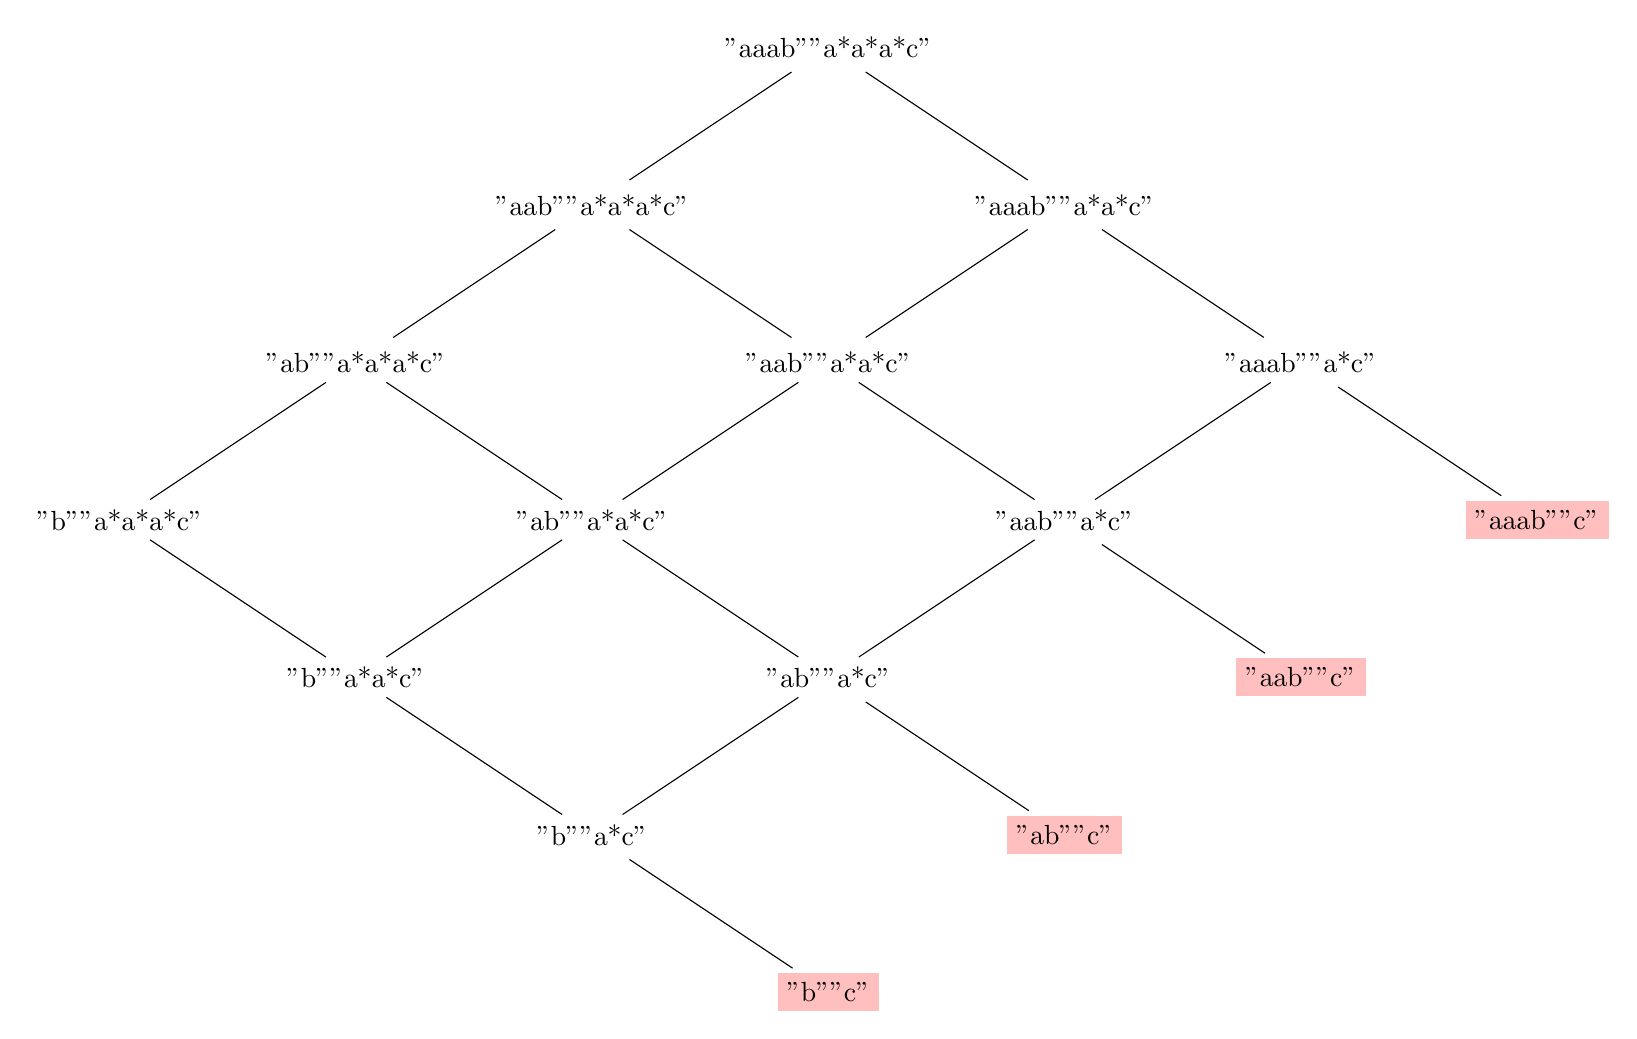
\begin{tikzpicture}[align=center, draw, black, shorten >=3pt, shorten <=3pt, node distance = 2.5cm]
  \node at (5, 0) (root) {\state{"aaab"}{"a*a*a*c"}};

  \node at (2, -2) (L) {\state{"aab"}{"a*a*a*c"}};
  \node at (8, -2) (R) {\state{"aaab"}{"a*a*c"}};

  \draw (root) -- (L);
  \draw (root) -- (R);

  \node at (-1, -4) (LL) {\state{"ab"}{"a*a*a*c"}};
  \node at (5, -4) (mid1) {\state{"aab"}{"a*a*c"}};
  \node at (11, -4) (RR) {\state{"aaab"}{"a*c"}};

  \draw (L) -- (LL);
  \draw (R) -- (RR);
  \draw (L) -- (mid1);
  \draw (R) -- (mid1);

  \node at (-4, -6) (LLL) {\state{"b"}{"a*a*a*c"}};
  \node at (2, -6) (mid2L) {\state{"ab"}{"a*a*c"}};
  \node at (8, -6) (mid2R) {\state{"aab"}{"a*c"}};
  \node[fill=red!25] at (14, -6) (RRR) {\state{"aaab"}{"c"}};

  \path[draw, black]
  (LL) -- (LLL)
  (LL) -- (mid2L)
  (mid1) -- (mid2L)
  (mid1) -- (mid2R)
  (RR) -- (mid2R)
  (RR) -- (RRR)
  ;

  % \node[rectangle, dashed, draw=none] at (-7, -8) (LLLL) {\state{"b"}{"a*a*c"}};
  \node at (-1, -8) (mid3-1) {\state{"b"}{"a*a*c"}};
  \node at (5, -8) (mid3-2) {\state{"ab"}{"a*c"}};
  \node[fill=red!25] at (11, -8) (mid3-3) {\state{"aab"}{"c"}};
  % \node at (17, -8) (RRRR) {}; % also dead

  \path[draw, black]
  (LLL) -- (mid3-1)
  (mid2L) -- (mid3-1)
  (mid2L) -- (mid3-2)
  (mid2R) -- (mid3-2)
  (mid2R) -- (mid3-3)
  % (RRR) -- (mid3-3)
  ;

  \node at (2, -10) (mid4-1) {\state{"b"}{"a*c"}};
  \node[fill=red!25] at (8, -10) (mid4-2) {\state{"ab"}{"c"}};

  \path[draw, black]
  (mid3-1) -- (mid4-1)
  (mid3-2) -- (mid4-1)
  (mid3-2) -- (mid4-2)
  % (mid3-3) -- (mid4-2)
  ;

  \node[fill=red!25] at (5, -12) (mid5) {\state{"b"}{"c"}};

  \path[draw, black]
  (mid4-1) -- (mid5)
  % (mid4-2) -- (mid5)
  ;

\end{tikzpicture}
\end{document}

